\documentclass{article}
\usepackage{graphicx, fancyhdr, amsmath}
\usepackage[margin=0.6in, top=1in]{geometry}
\usepackage{float}
\usepackage[absolute, overlay]{textpos}
\usepackage[colorlinks=true, linkcolor=blue]{hyperref}

\pagestyle{fancy}
\fancyhf{}
\renewcommand{\headrulewidth}{0pt}

\fancyhead[L]{
\begin{textblock*}{2cm}(0.3in,0.1in)  % {block width} (x-coordinate, y-coordinate)
    
\includegraphics[width=2cm]{NEW LOGO.png}  % Example image placeholder
\end{textblock*}
}
\fancyhead[R]{Math Success Program, UCLA}
\fancyfoot[R]{Created for the MSP by Asmi Kawatkar}

\fancypagestyle{plain}{
}


\title{Review Sheet: L'Hopital's Rule}
\date{}
\author{}

\begin{document}
\maketitle
\vspace{-0.75in}
\section*{Content Review}
\subsection*{Overview}

L'Hopital's rule is a technique used to simplify the evaluation of limits. Note that it does not directly evaluate limits, but rather simplifies the process of evaluating limits. 
\vspace{10pt
}

\noindent \textit{When can we apply L'Hopital's Rule?}
\newline L'Hopital's Rule can only be applied in situations where the limit as it currently stands evaluates to one of the two following indeterminate forms:
$$\frac{0}{0} \hspace{10pt} \text{or} \hspace{10pt} \frac{\pm \infty}{\pm \infty}$$

Note that L'Hopitals rule \textbf{CANNOT} be applied if the limit evaluates to any of the following forms (or more generally, to any form that is not the above two):
$$\frac{0}{\pm \infty} \hspace{10pt} \text{or} \hspace{10pt} \frac{\pm \infty}{0} \hspace{10pt} \text{or} \hspace{10pt} \frac{1}{\pm \infty} \hspace{10pt} \text{or} \hspace{10pt} \frac{\pm \infty}{1}  \hspace{10pt} \text{or} \hspace{10pt} \frac{1}{0}$$

\noindent \textit{How to apply L'Hopital's Rule?}
\newline Suppose we want to evaluate
$$\lim_{x \rightarrow a}\frac{f(x)}{g(x)}$$
where the limit $a$ could be an ordinary number or $\pm \infty$. Provided that the limit satisfies one of the two indeterminate forms shown above, we can apply L'Hopital's Rule to state that:

$$\lim_{x \rightarrow a}\frac{f(x)}{g(x)} = \lim_{x \rightarrow a}\frac{f'(x)}{g'(x)}$$

\noindent Note that this is not the same as applying the quotient rule. 

\subsection*{Resources}


\noindent\textit{L'Hopital's Rule}
\begin{itemize}
    \item \href{https://youtu.be/Gh48aOvWcxw}{Video: L'Hopital's Rule (Organic Chemistry Tutor, 13 min) - with worked examples} 
    \item \href{https://tutorial.math.lamar.edu/classes/calci/lhospitalsrule.aspx}{Content \& Worked Examples (Paul's Online Notes)}
    \item \href{https://www.khanacademy.org/math/ap-calculus-ab/ab-diff-contextual-applications-new/ab-4-7/v/introduction-to-l-hopital-s-rule}{L'Hopital's Rule (Khan Academy Module)}
    \item \href{https://www.math.ucdavis.edu/~kouba/CalcOneDIRECTORY/lhopitaldirectory/LHopital.html}{Practice Problems: L'Hopital's Rule (UC Davis Math) - has worked solutions}
    \item \href{https://ic.arc.losrios.edu/~mirzaam/math400/LHOPITALRULE.pdf}{Content \& Worked Examples (Textbook)}
\end{itemize}


\subsection*{Acknowlegement}
Questions in the Worked Problems section of this sheet have been taken from external sources that have been linked where appropriate. All solutions have been created independently.

\pagebreak
\section*{Worked Problems}
\label{WorkedProblems}
\href{https://www.math.cmu.edu/~bkell/lhopital.pdf}{Source} and another \href{https://www.murrieta.k12.ca.us/cms/lib/CA01000508/Centricity/Domain/1702/LHopitals%20rule%20overview%20and%20practice.pdf}{Source}
\newline \noindent Find the following limits. You may use L'Hopital's rule where appropriate. Note that L'Hopital's rule may not apply to every limit, and it may not be helpful even when it does apply. 

\begin{enumerate}
    \item $$\lim_{x\rightarrow - \infty}\frac{3x-1}{x^2 + 1}$$
    \begin{figure}[H]
        \centering
        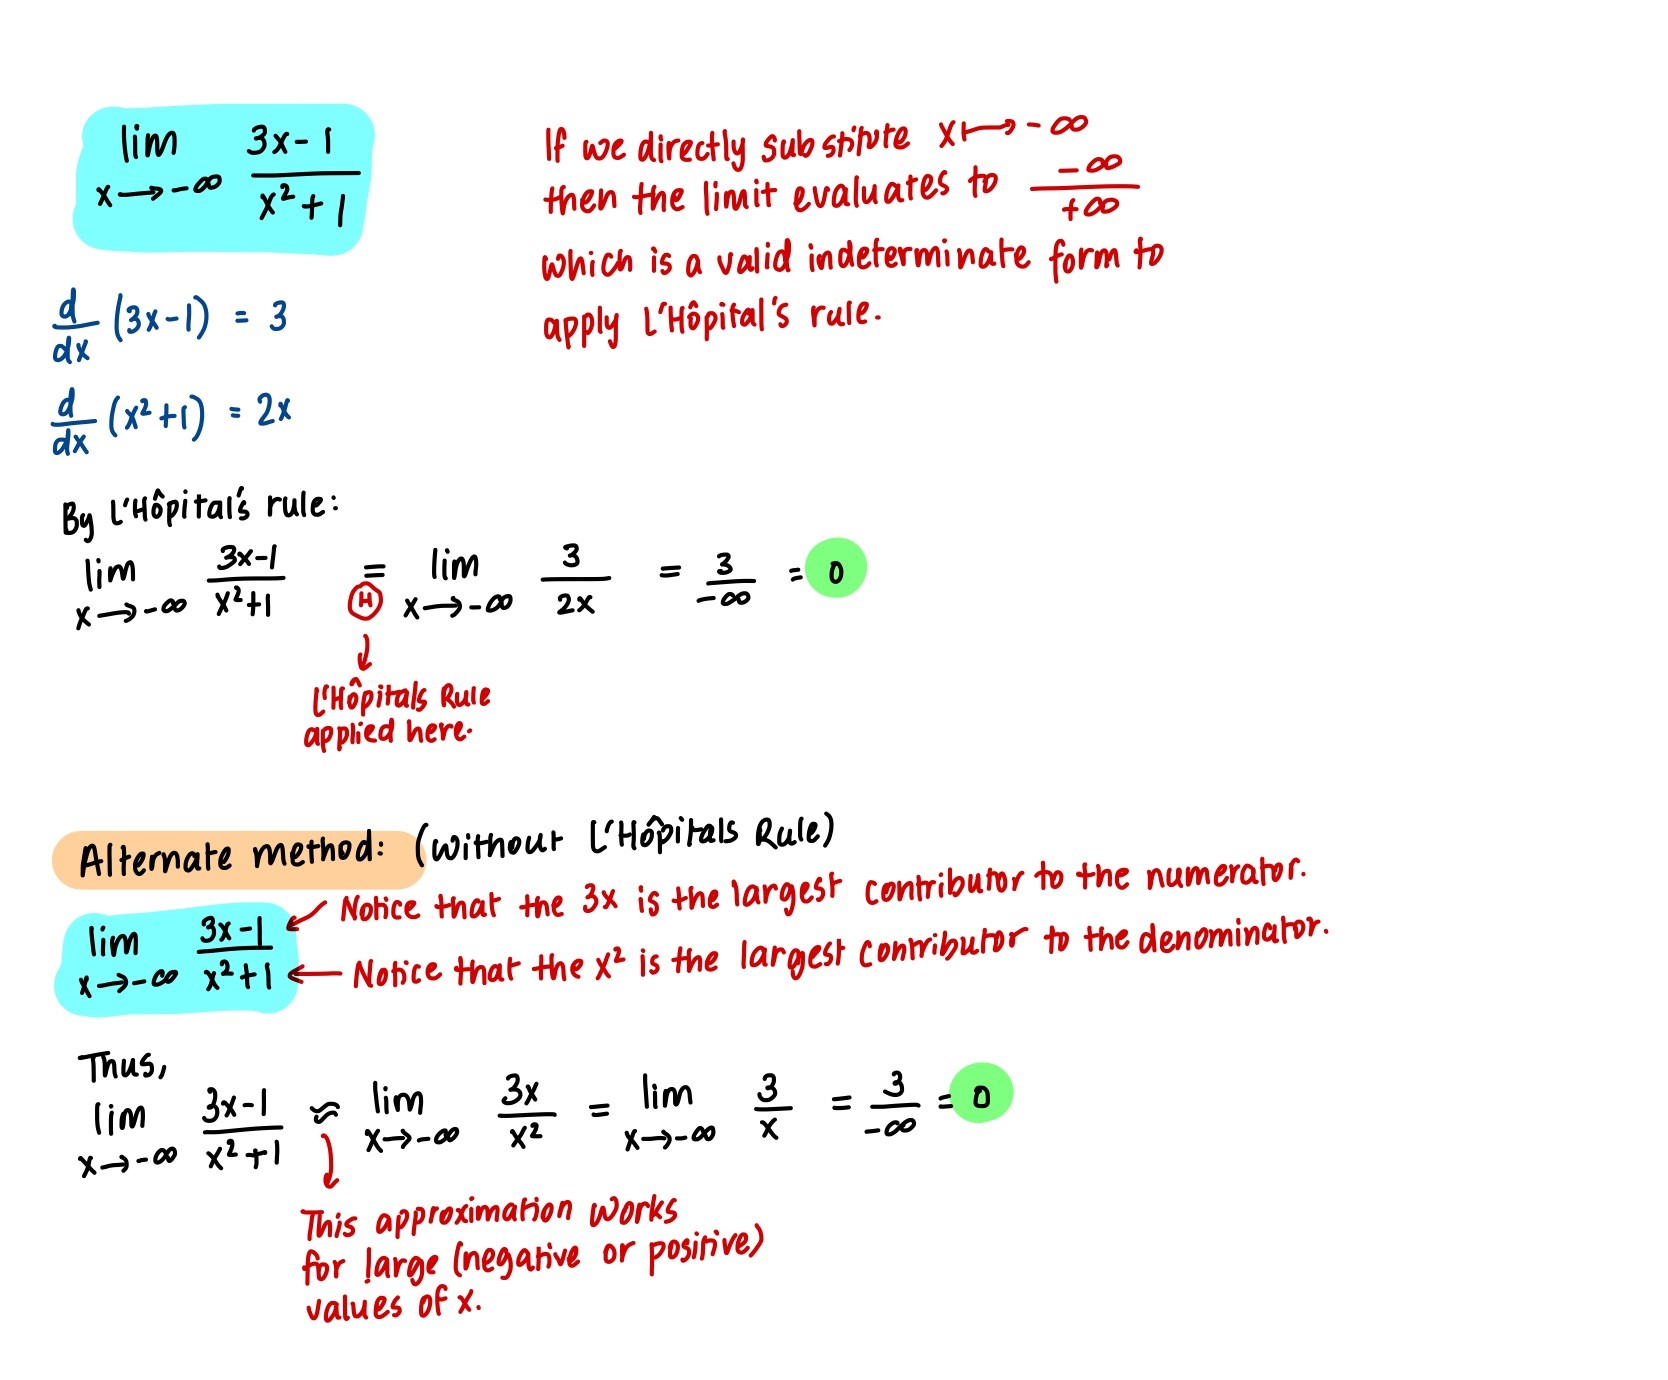
\includegraphics[width=\linewidth]{Q1.jpg}
        \label{fig:Q1}
    \end{figure}
    \newpage
    \item $$\lim_{x \rightarrow 0}\frac{e^x-x-1}{\cos x - 1}$$
    \begin{figure}[H]
        \centering
        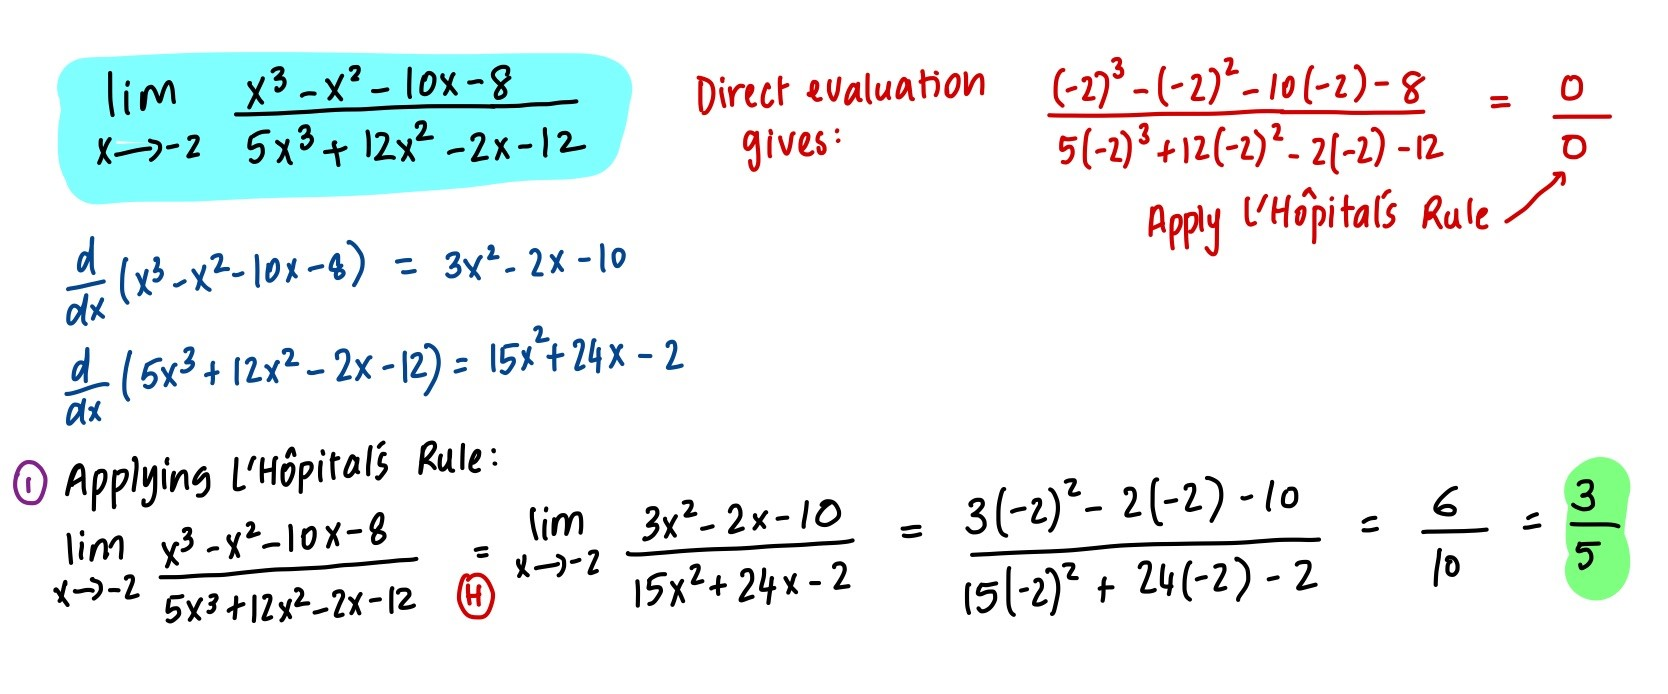
\includegraphics[width=\linewidth]{Q2.jpg}
        \label{fig:Q2}
    \end{figure}
    \item $$\lim_{x \rightarrow -2}\frac{x^3-x^2-10x-8}{5x^3+12x^2-2x-12}$$
    \begin{figure}[H]
        \centering
        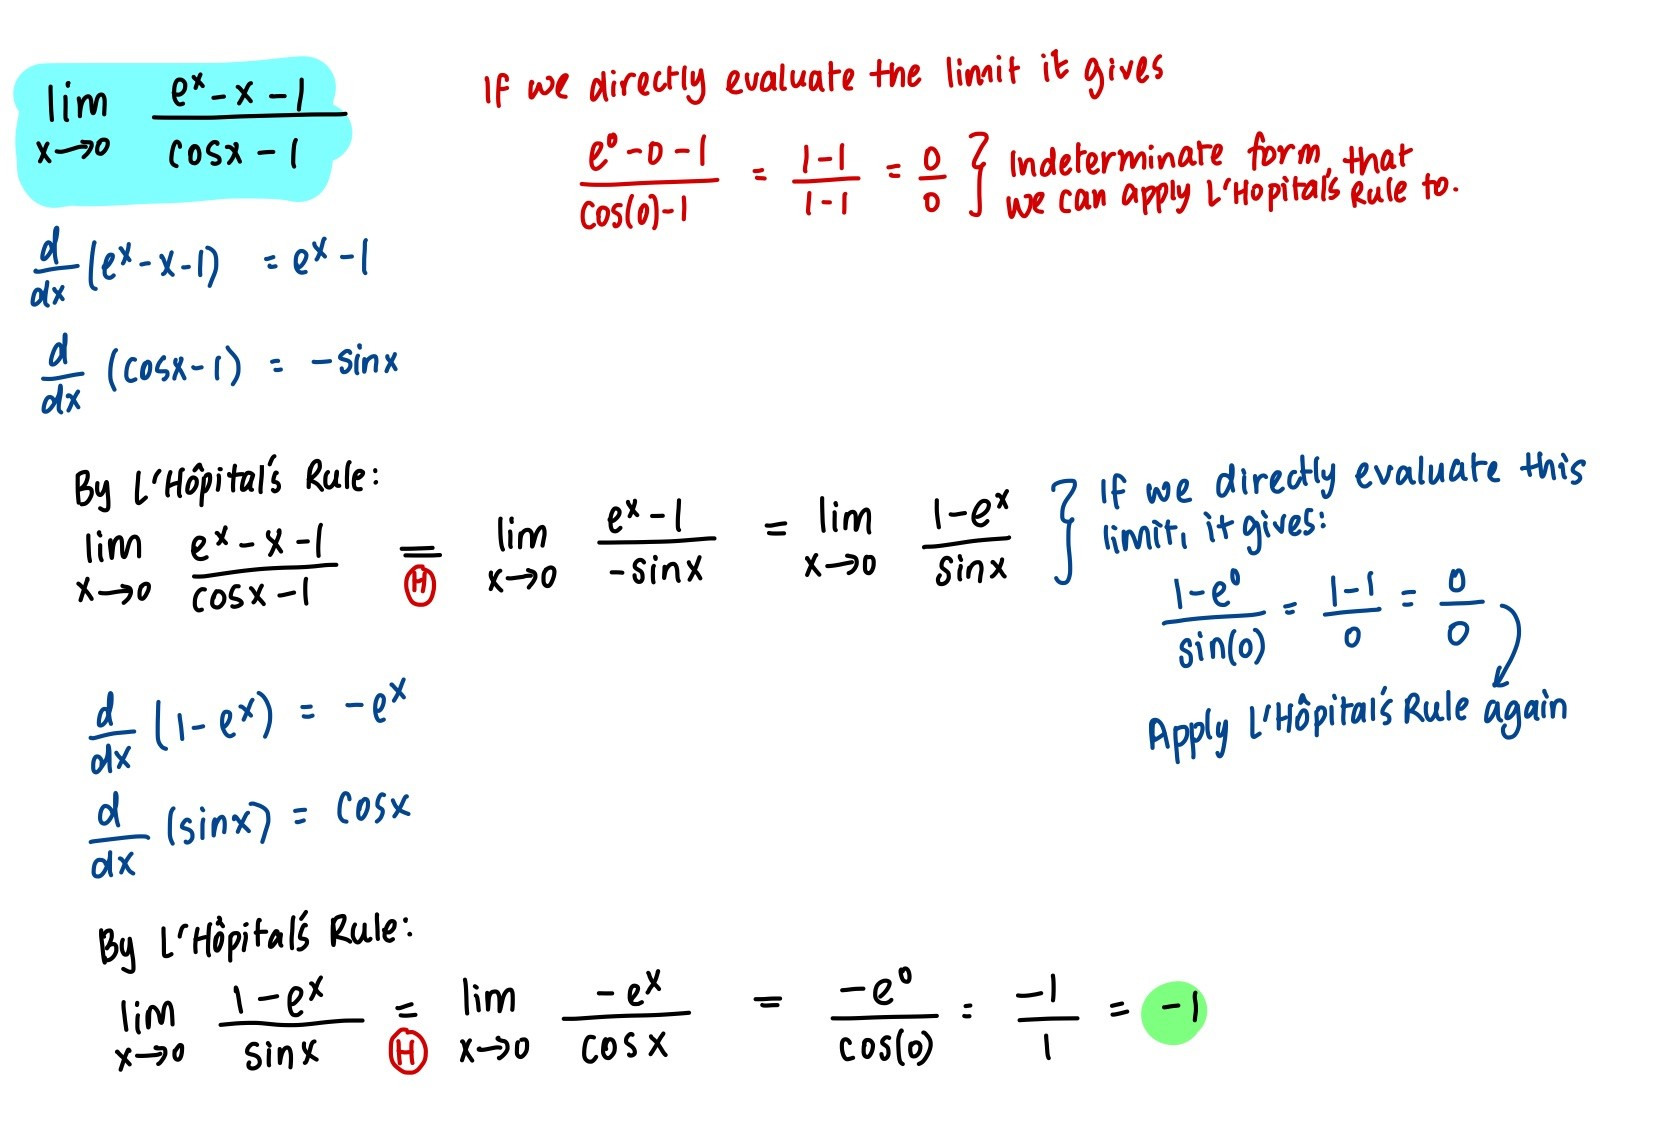
\includegraphics[width=0.9\linewidth]{Q3.jpg}
        \label{fig:Q3}
    \end{figure}
    \item $$\lim_{x \rightarrow 0}  \frac{\sin(6x)}{\sin(3x)}$$
    \begin{figure}[H]
        \centering
        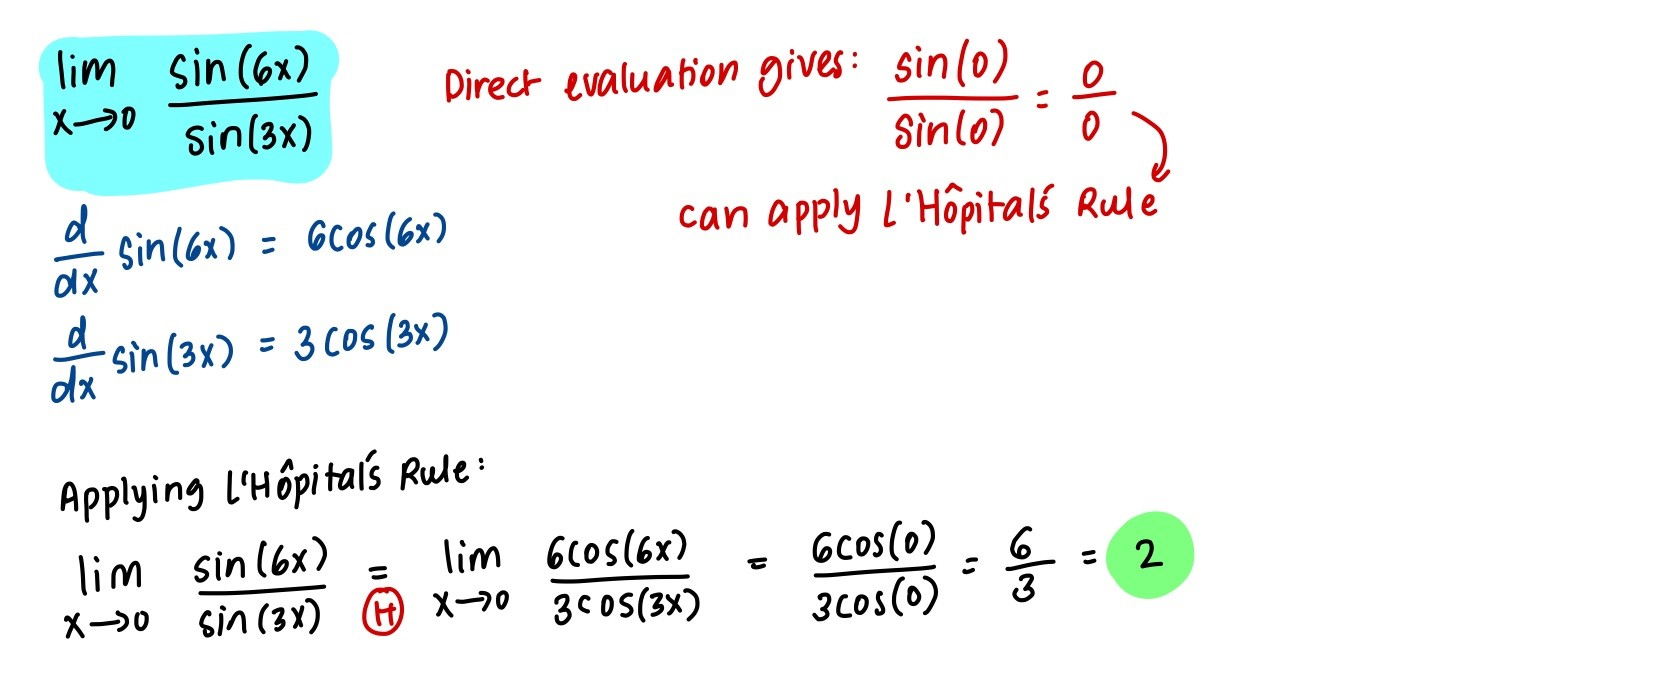
\includegraphics[width=\linewidth]{Q4.jpg}
        \label{fig:Q4}
    \end{figure}
    \item $$\lim_{x \rightarrow 1} \frac{\ln x^2}{9x^2-9}$$
    \begin{figure}[H]
        \centering
        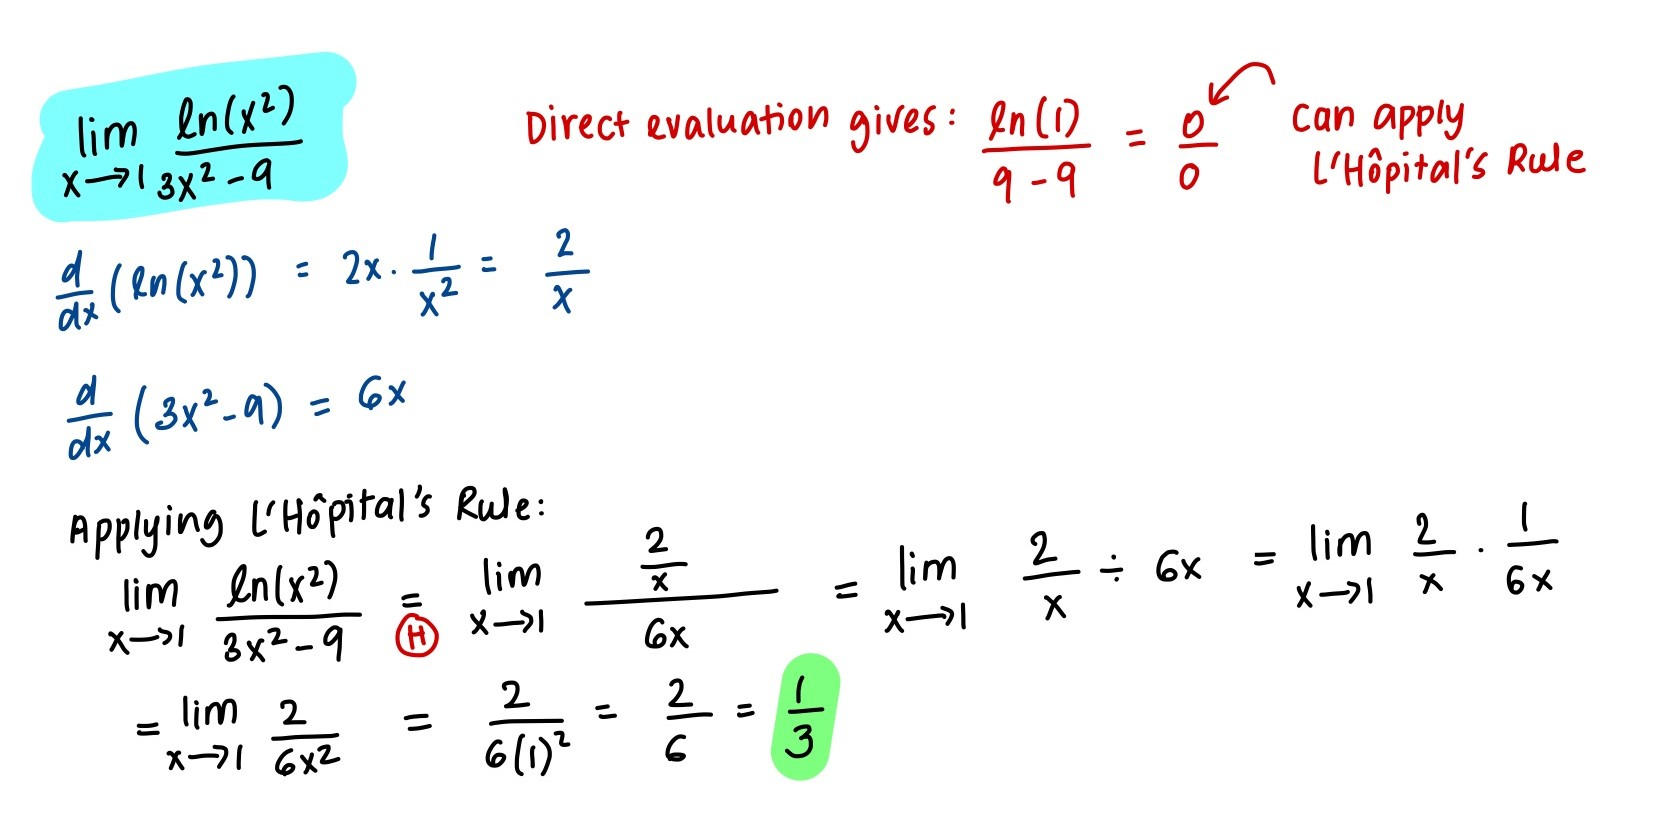
\includegraphics[width=\linewidth]{Q5.jpg}
        \label{fig:Q5}
    \end{figure}
    \newpage
    \item $$\lim_{x \rightarrow 0}\frac{\tan x - x}{x^3}$$
    \begin{figure}[H]
        \centering
        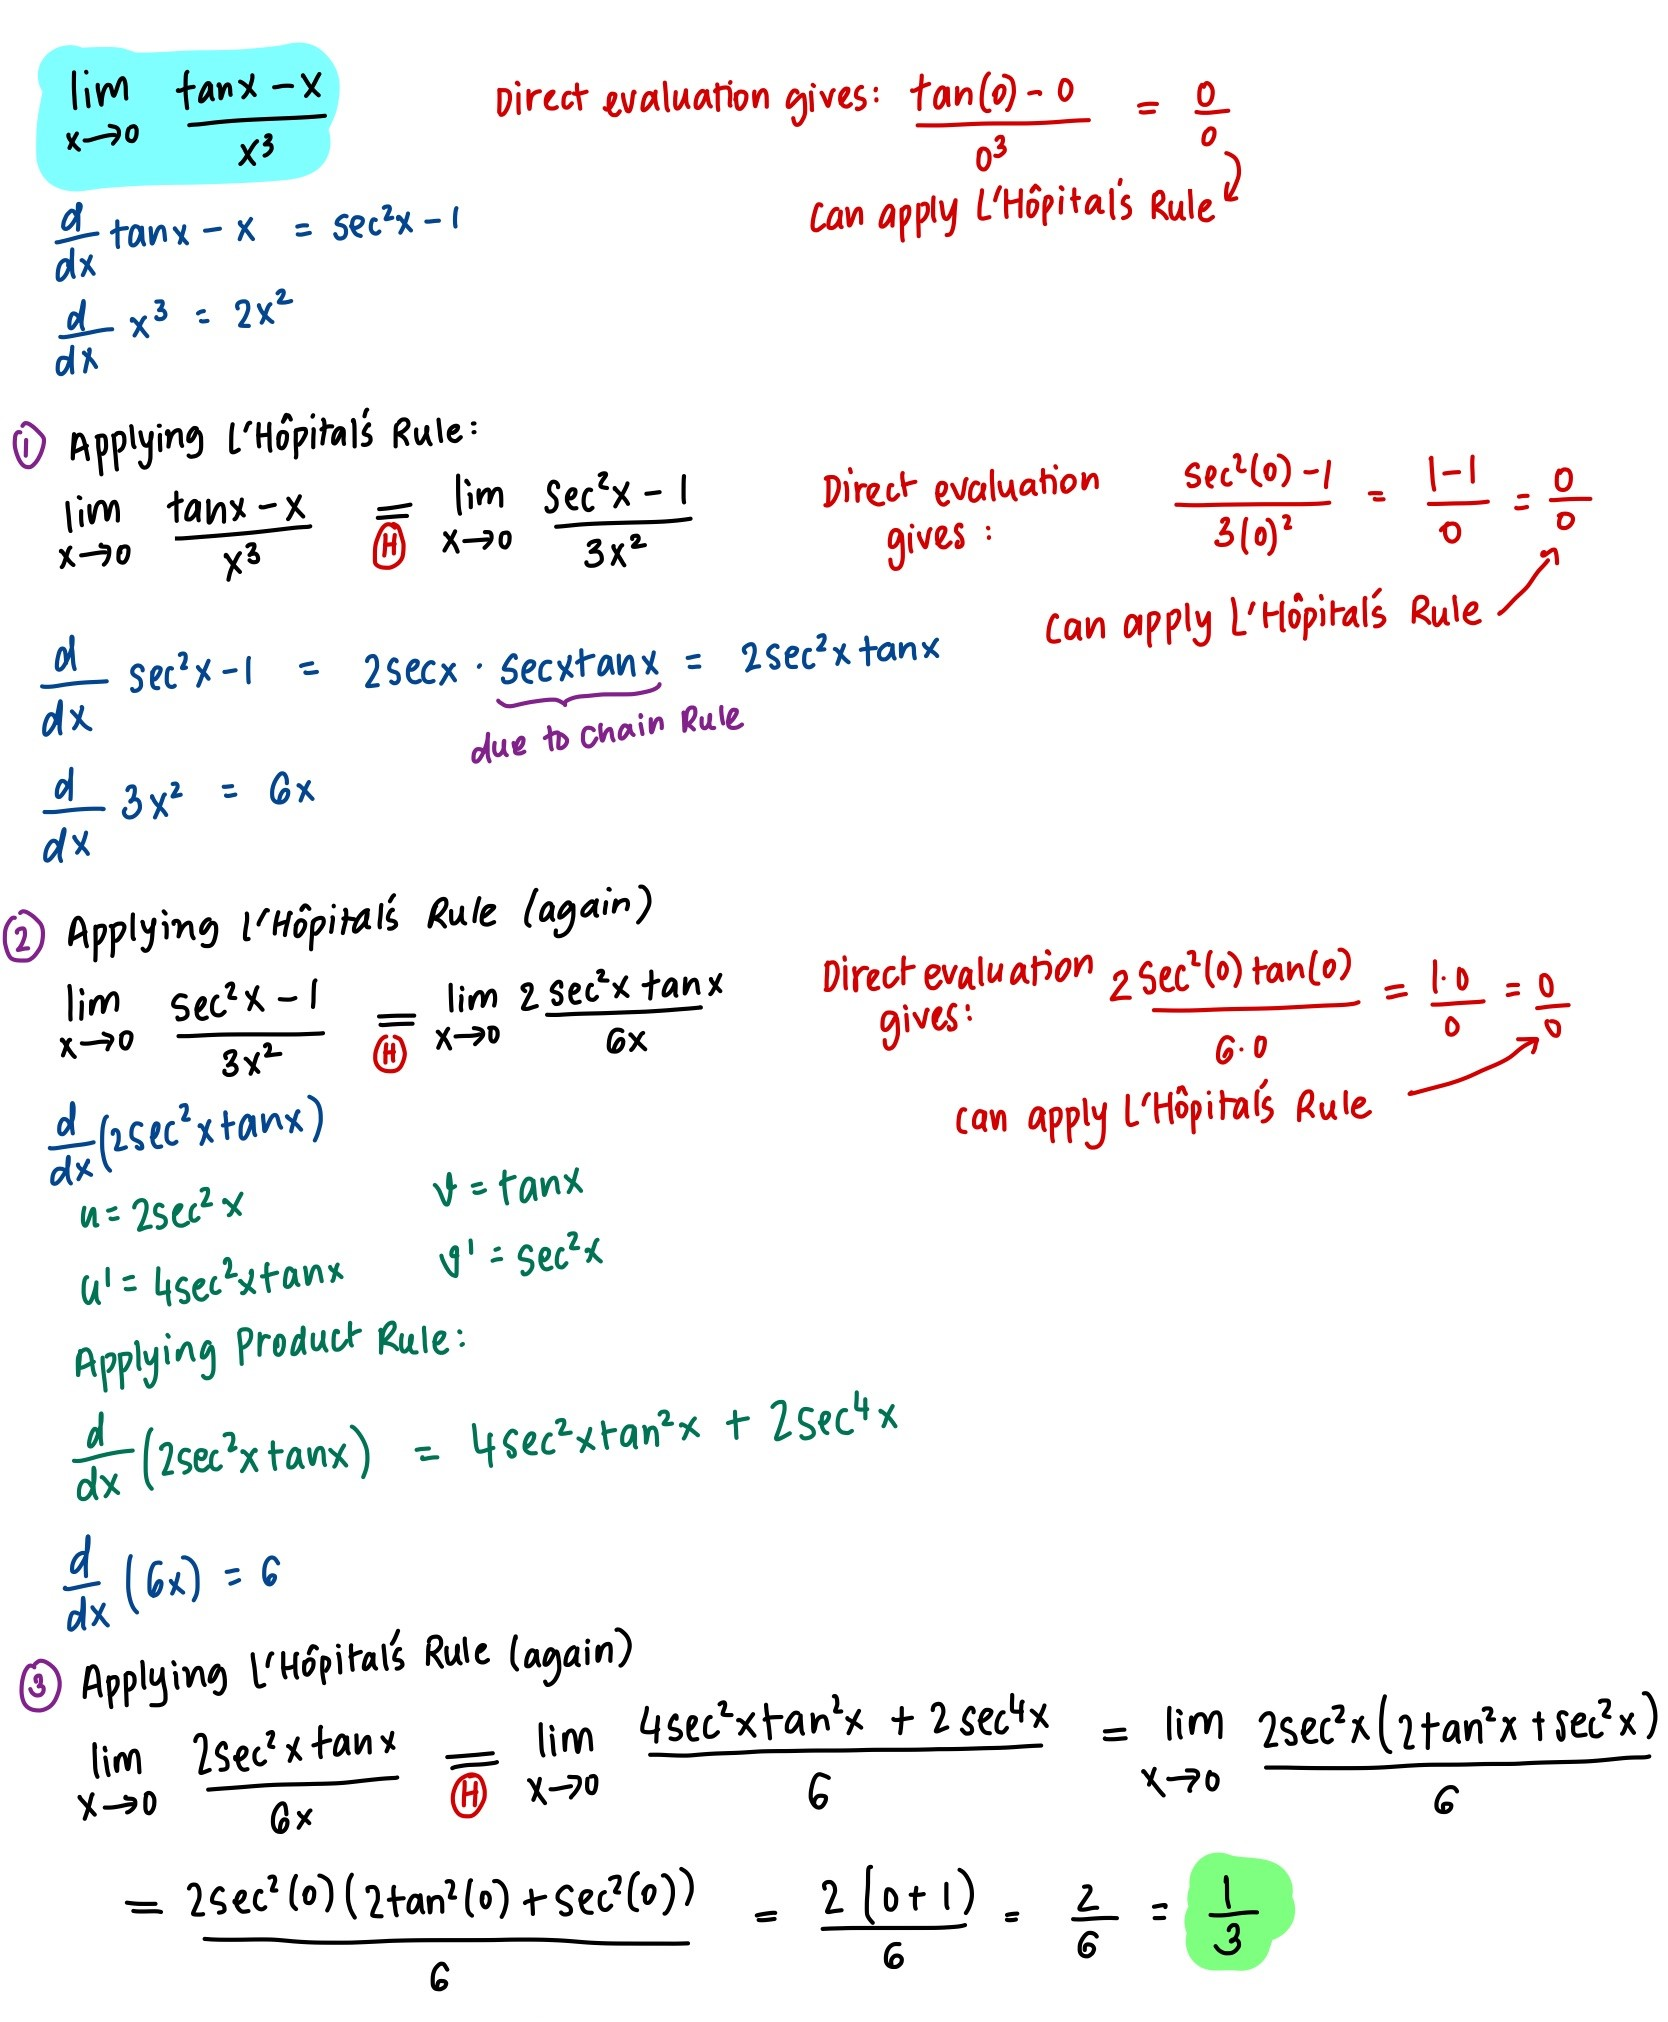
\includegraphics[width=0.95\linewidth]{Q6.jpg}
        \label{fig:Q6}
    \end{figure}
    \item $$\lim_{x \rightarrow 0}\frac{\sin x - x}{x^3}$$
    \begin{figure}[H]
        \centering
        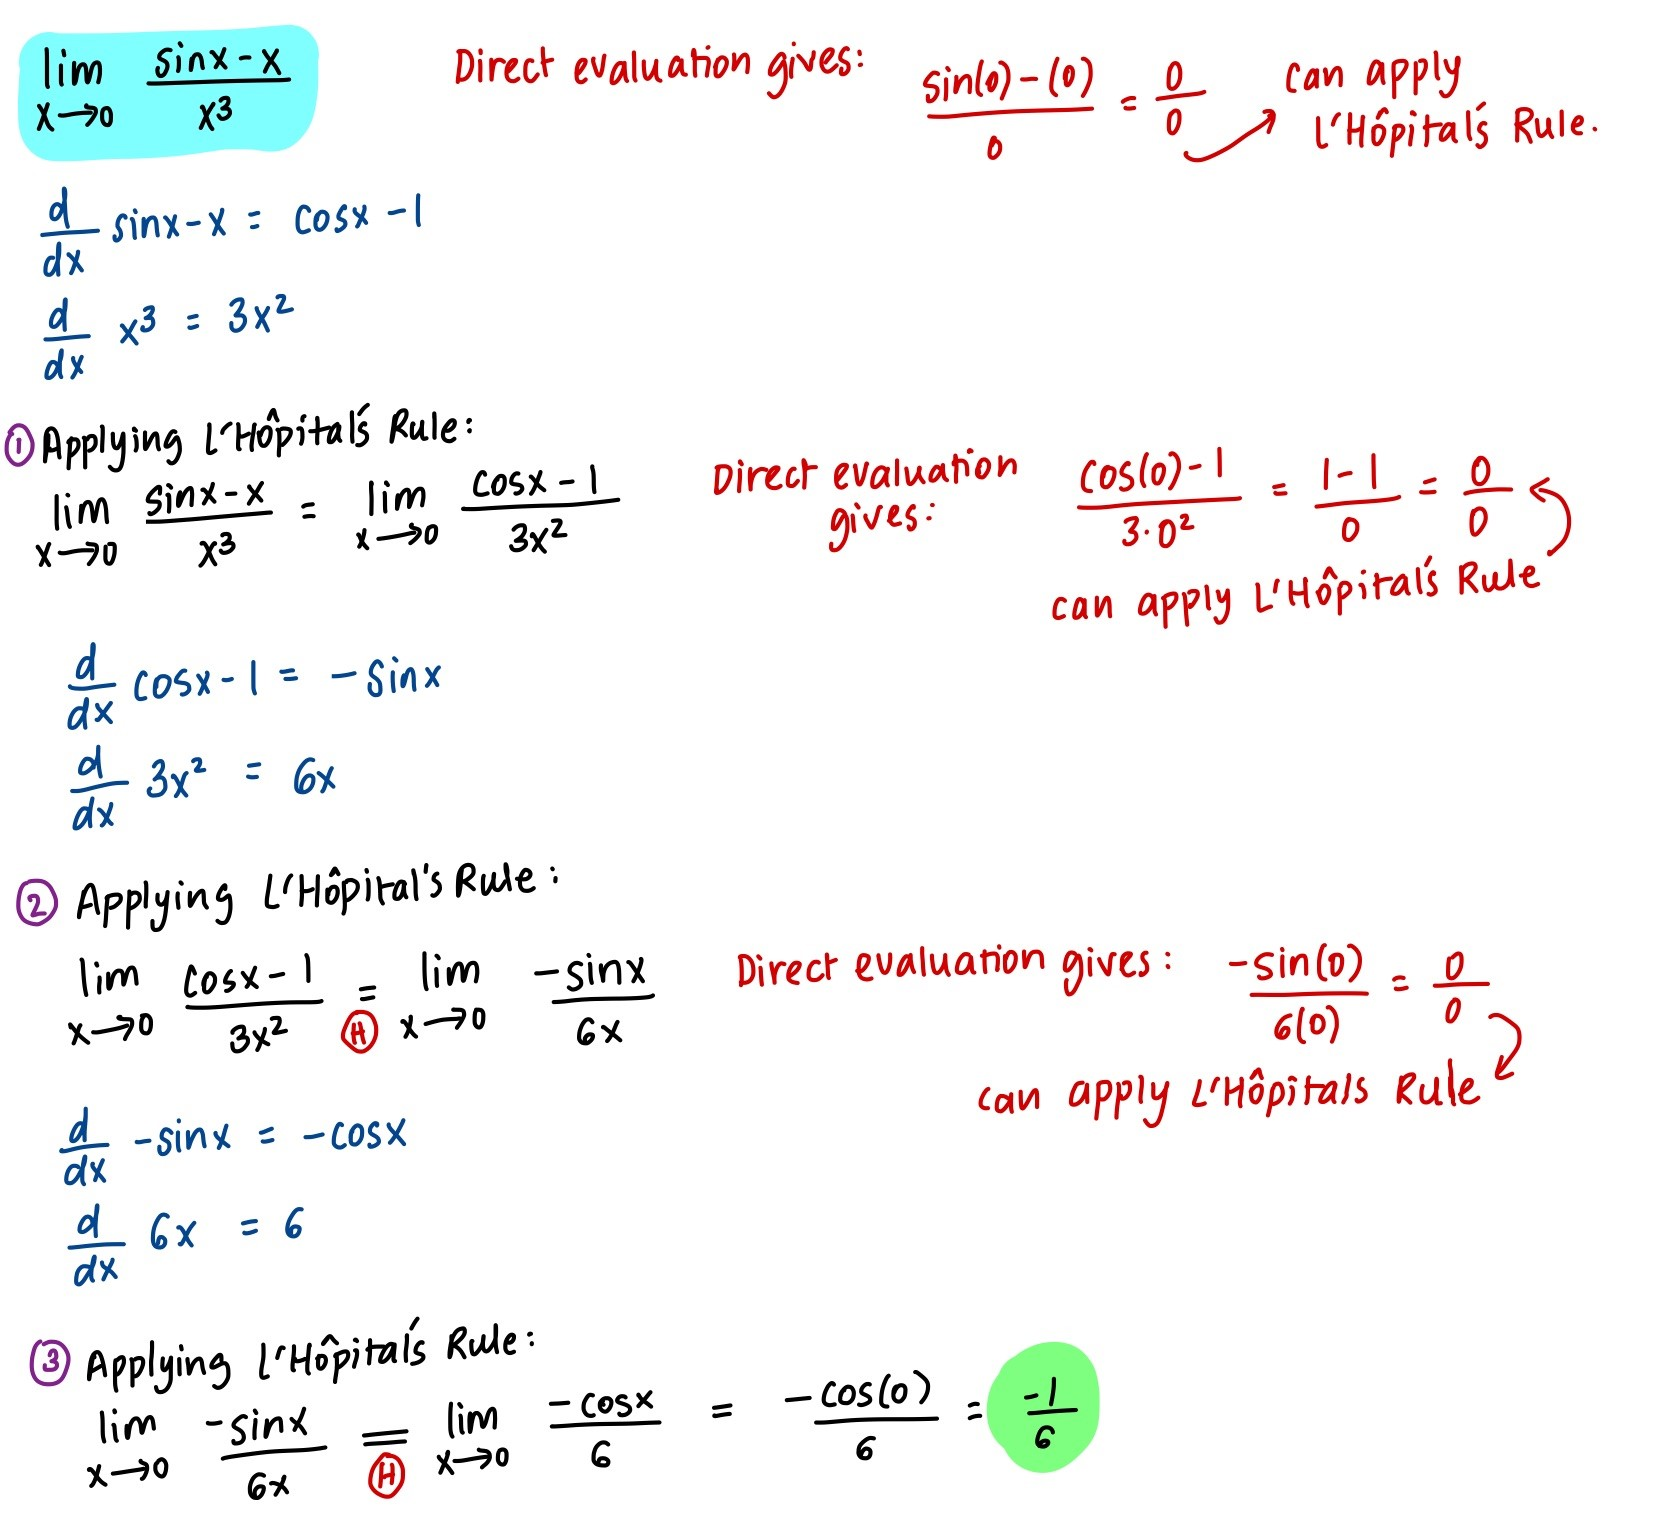
\includegraphics[width=0.9\linewidth]{Q7.jpg}
        \label{fig:Q7}
    \end{figure}
    \newpage
    \item $$\lim_{x \rightarrow 0}x\sin{\frac{1}{x}}$$
    \begin{figure}[H]
        \centering
        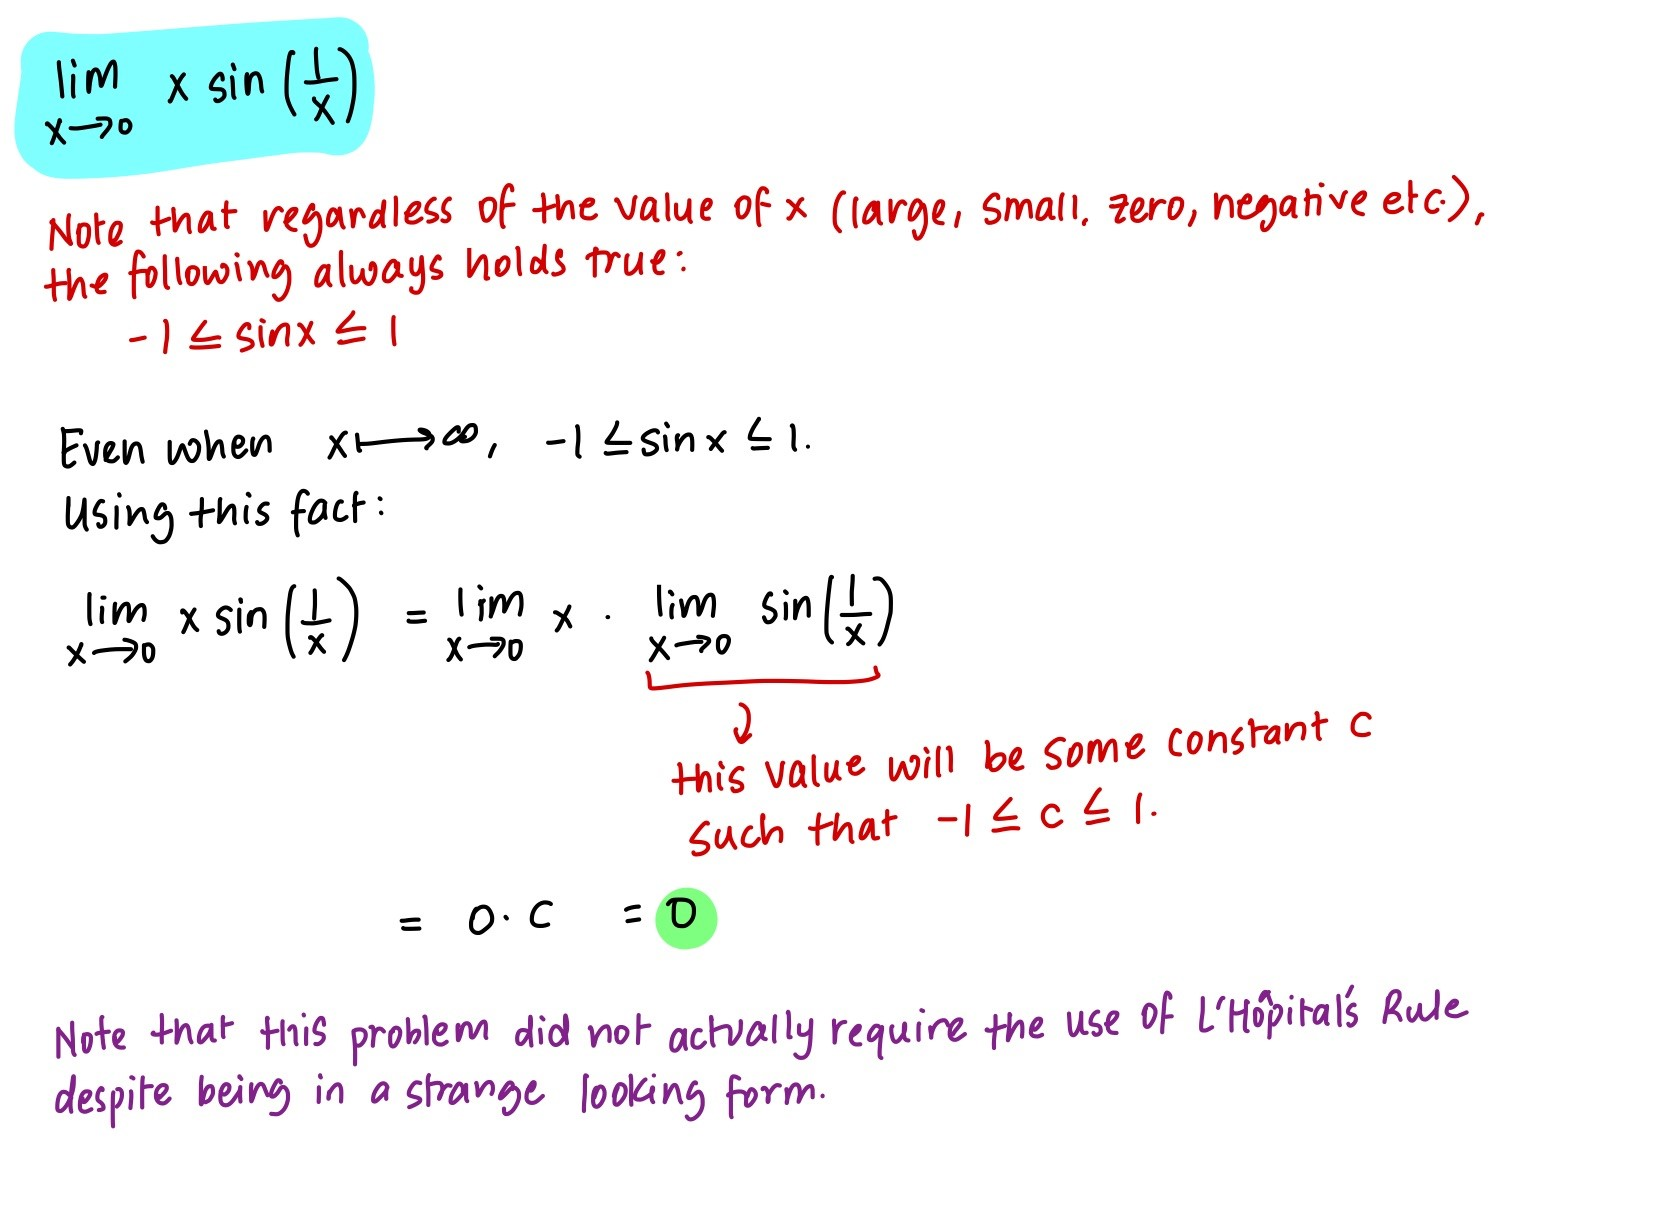
\includegraphics[width=0.9\linewidth]{Q8.jpg}
        \label{fig:Q8}
    \end{figure}
    \newpage
    \item $$\lim_{x\rightarrow + \infty}\frac{\ln(x^2+1)}{\ln(x^3+1)}$$
    \begin{figure}[H]
        \centering
        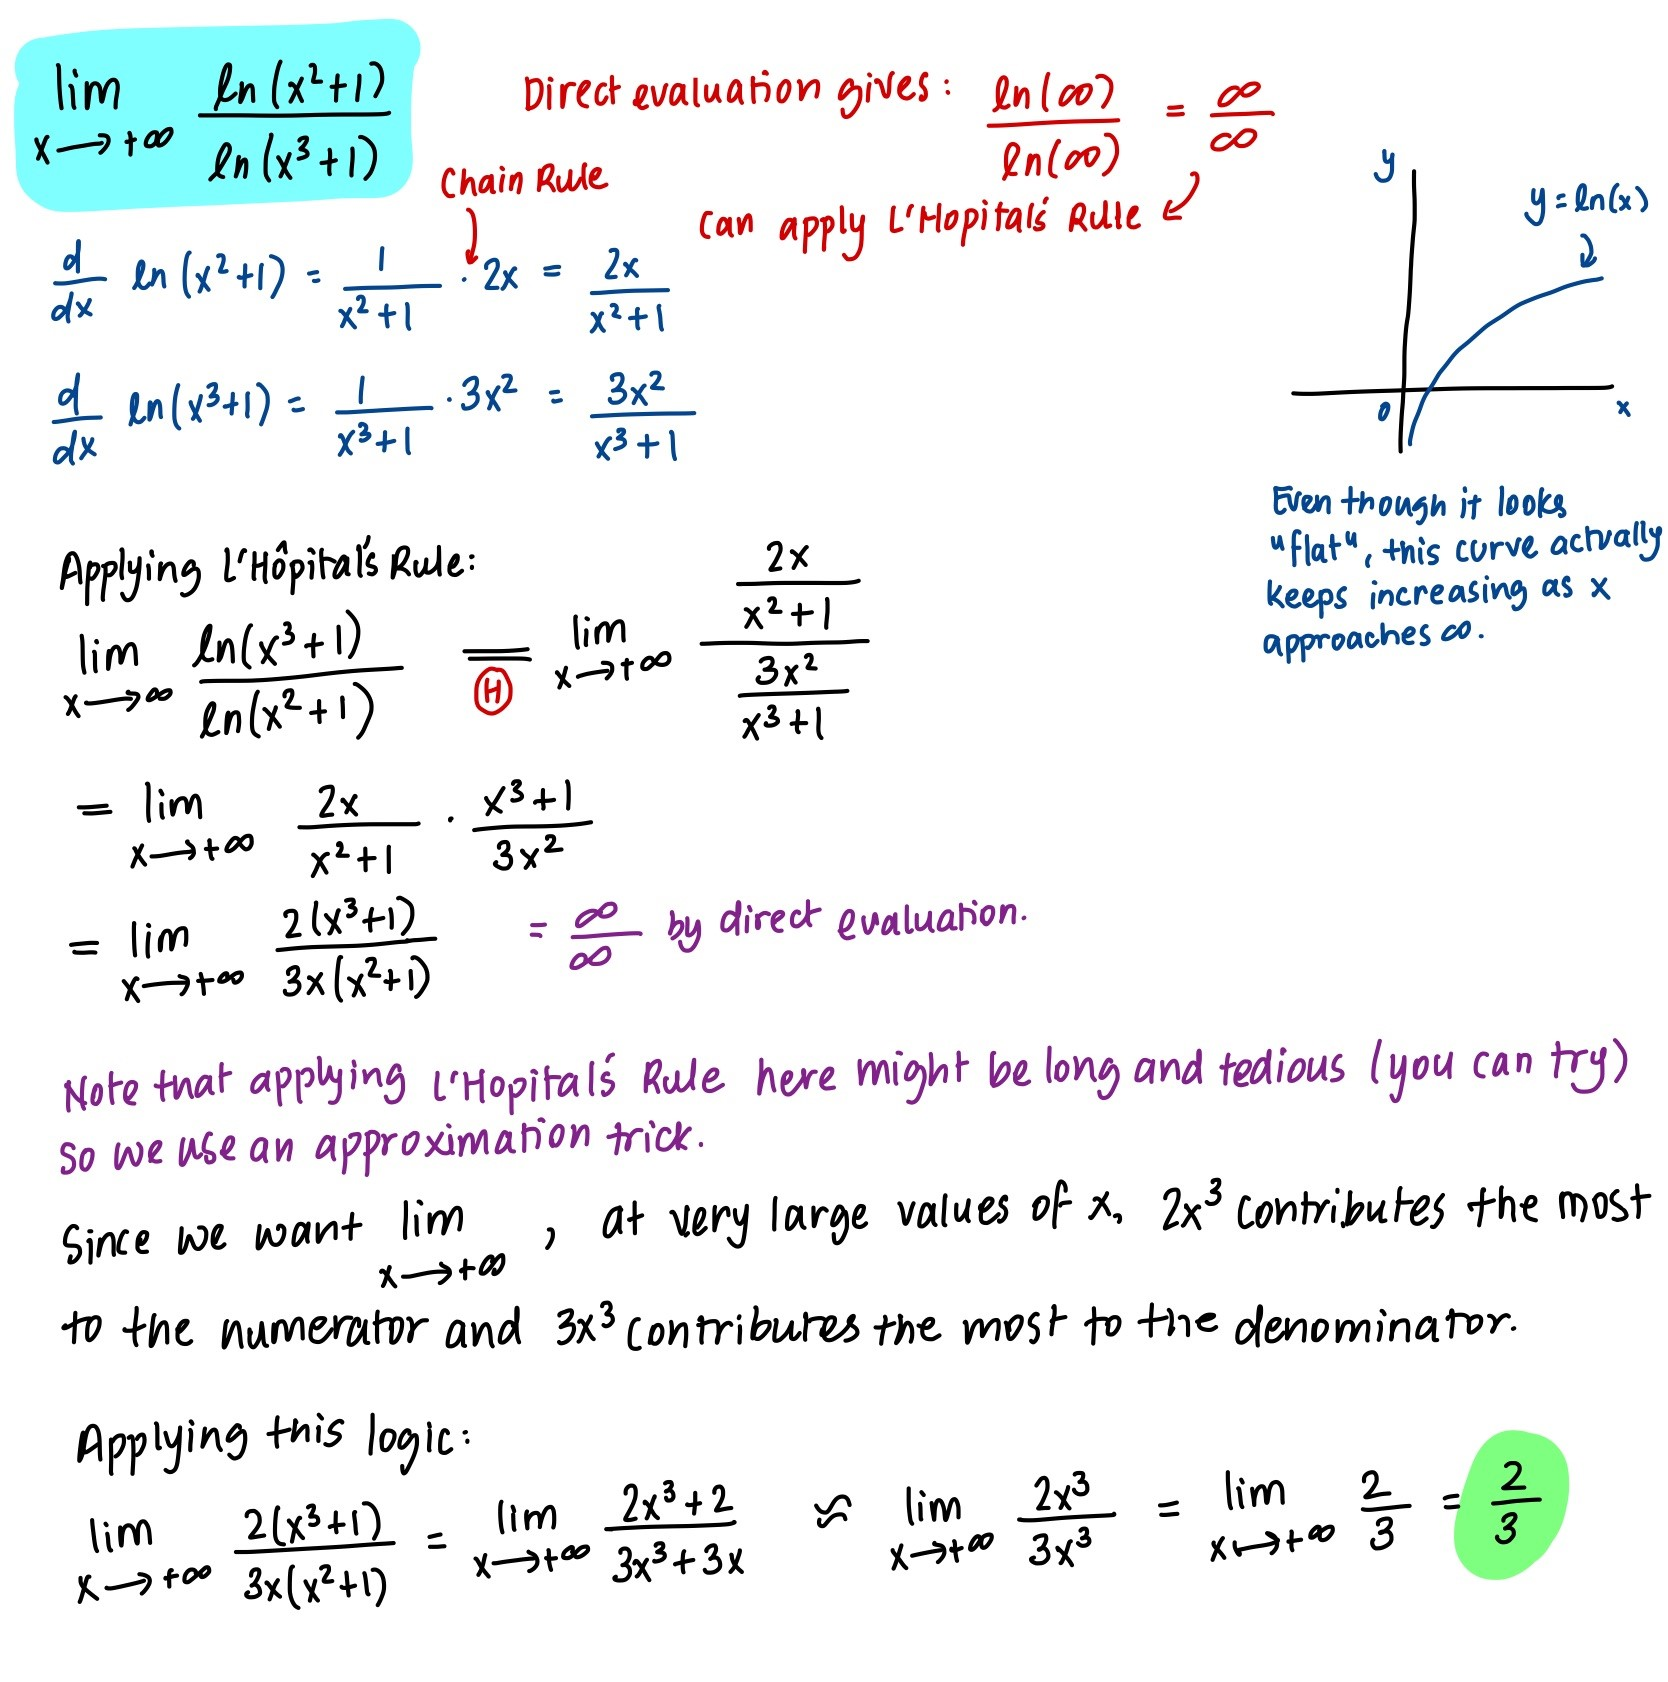
\includegraphics[width=\linewidth]{Q9.jpg}
        \label{fig:Q9}
    \end{figure}
    \newpage
    \item $$\lim_{x \rightarrow 0}\frac{xe^{3x}-x}{1-\cos(2x)}$$
    \begin{figure}[H]
        \centering
        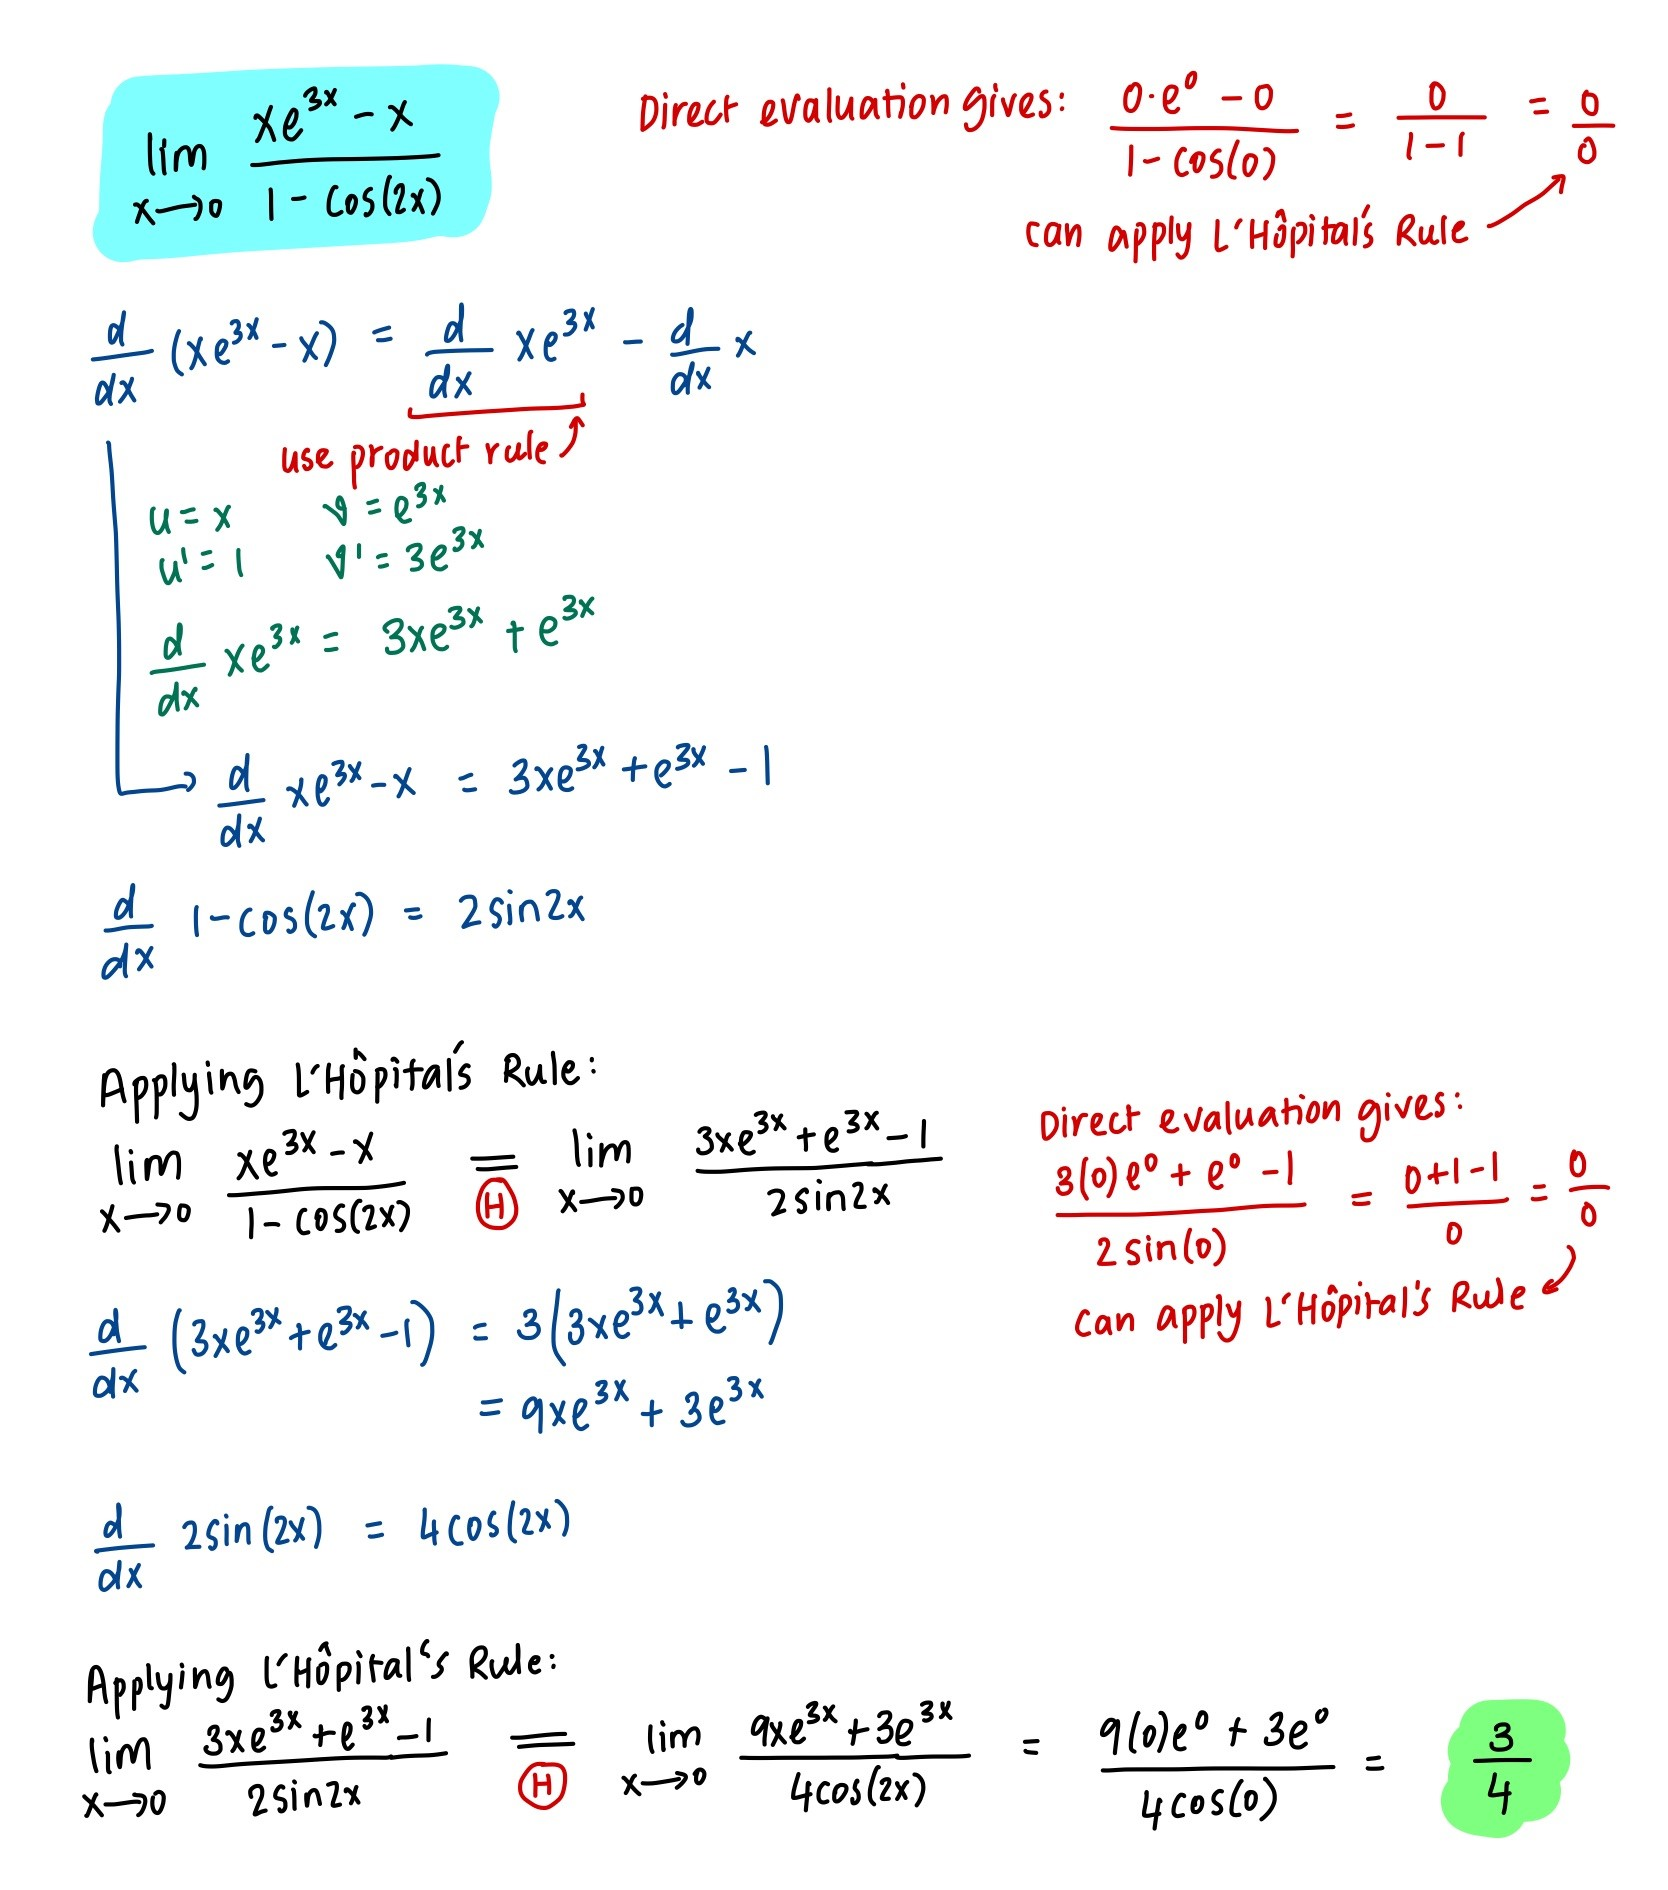
\includegraphics[width=\linewidth]{Q10.jpg}
        \label{fig:Q10}
    \end{figure}
\end{enumerate}

\end{document}
